\chapter{Sensing, Subsampling and interpolation}%
\label{chap:02}
\setcounter{section}{1}

\paragraph{Summary} This week's lecture is concerned with downsampling and
upsampling. We show that the na\"\i{}ve approaches should not be used and
discuss the different alternatives that should be applied. Further, we discuss
how the operations can be written in terms of matrix multiplications.

\section{On Downsampling}
To deal with very large images one often needs to downsample the image so that
it fits into the memory of the GPU. Within the context of neural networks, one
approach is to feed only a small patch of the image into the network. Of course,
the network then ignores everything outside of this patch, even when we
``slide'' the small patch across the image. Another approach that makes use of
the information across the whole image is to downsample the image. The
\emph{wrong} appproach would be to take the first pixels, then leave out a fixed
number, then take the next pixel and repeat (see lecture notebook for an
example). The correct way would be to first smooth (blur) the image and only
then subsample.

The effect of the na\"\i{}ve approach can be explained as follows. Subsampling
is a linear operation and can thus be written as a matrix multiplication. If we
denote by a preceding downwards arrow the signal after subsampling, we can write
\begin{equation*}
  \downarrow g = h =
  \begin{bmatrix}
    1 & 0 & 0 & 0 & 0 & 0 & 0 & 0 \\
    0 & 0 & 1 & 0 & 0 & 0 & 0 & 0 \\
    0 & 0 & 0 & 0 & 1 & 0 & 0 & 0 \\
    0 & 0 & 0 & 0 & 0 & 0 & 1 & 0
  \end{bmatrix}
  \cdot
  \begin{bmatrix}
    g_0 \\ g_1 \\ \vdots \\ g_7
  \end{bmatrix}\,.
\end{equation*}
Every other sample is \textbf{completely lost}! Idea: Average two adjacent
samples. This can be written as a convolution of a blur $b$ with the signal $g$
\begin{equation*}
  \downarrow (b \ast g) = h^\prime = \frac{1}{2}
  \begin{bmatrix}
    1 & 1 & 0 & 0 & 0 & 0 & 0 & 0 \\
    0 & 0 & 1 & 1 & 0 & 0 & 0 & 0 \\
    0 & 0 & 0 & 0 & 1 & 1 & 0 & 0 \\
    0 & 0 & 0 & 0 & 0 & 0 & 1 & 1
  \end{bmatrix}
  \cdot
  \begin{bmatrix}
    g_0 \\ g_1 \\ \vdots \\ g_7
  \end{bmatrix}
  =
  \begin{bmatrix}
    \frac{1}{2} g_0 + \frac{1}{2} g_1 \\
    \frac{1}{2} g_2 + \frac{1}{2} g_3 \\
    \vdots \\
    \frac{1}{2} g_6 + \frac{1}{2} g_7
  \end{bmatrix}\,.
\end{equation*}
All observations contribute to the result, \ie less information is lost. There
are also other approaches; for periodic boundary conditions, the following
matrix could be used
\begin{equation*}
  \frac{1}{4}
  \begin{bmatrix}
    2 & 1 & 0 & 0 & 0 & 0 & 0 & 1 \\
    0 & 1 & 2 & 1 & 0 & 0 & 0 & 0 \\
    0 & 0 & 0 & 1 & 2 & 1 & 0 & 0 \\
    0 & 0 & 0 & 0 & 0 & 1 & 2 & 1
  \end{bmatrix}\,,
\end{equation*}
which has some nice properties such as constant row and columns sums; also,
unlike the previous filters, this filter is symmetric around the particular
target sample.

We could take more samples around the target sample into account (fewer zero
entries per the rows) which gives rise to the question of whether or not there
optimal filters exist? In general, these filters will be data-dependent (this
essentially is PCA), \ie different filters for different data sets. To obtain a
generally appllicable filter which is not data-dependent, we need to make some
assumptions. A typical choice would be to assume the signal to be mostly
low-pass (such filters will predominantly preserve low frequencies; we therefore
assume the signal mostly consists of low frequencies). A perfect low-pass filter
\begin{itemize}
\item eliminates all frequencies above the new Nyquist limit (highest frequency
  that can be represented by sampling a signal uniformly), and
\item leaves frequencies below the Nyquist limit completely untouched.
\end{itemize}
The optimal choice is (no proof given)
\begin{equation*}
  \text{sinc}\,x = \frac{\sin \pi x}{\pi x}\,.
\end{equation*}
A plot is given in Figure~\ref{fig:sinc}. A possible discrete filter that we
would use for discrete signals could then be approximately
\begin{equation*}
  \left[ 0 \quad -\tfrac{1}{5} \quad 0 \quad \tfrac{2}{3} \quad 1 \quad \tfrac{2}{3} \quad 0 \quad -\tfrac{1}{5} \quad 0 \right]
\end{equation*}

\begin{figure}[h!]
\centering
\begin{tikzpicture}
\pgfmathdeclarefunction{sinc}{1}{%
\pgfmathparse{abs(#1)<0.01 ? int(1) : int(0)}%
  \ifnum\pgfmathresult>0 \pgfmathparse{1}\else\pgfmathparse{sin(#1 r)/#1}\fi%
}
\draw[->] (-4, 0) -- (4, 0);
\draw[->] (0, -1) -- (0, 3);
\draw[domain=-3:3, smooth, variable=\x, samples=250] plot ({\x},{2.5*sinc(8*\x)});

\draw[-{Circle[red]}, red, thick] (0,0) -- (0,2.5);
\draw[-{Circle[red]}, red, thick] (0.19,0) -- (0.19,1.66);
\draw[-{Circle[red]}, red, thick] (-0.19,0) -- (-0.19,1.66);

\filldraw[red] (0.38,0) circle (2pt);
\filldraw[red] (-0.38,0) circle (2pt);

\draw[-{Circle[red]}, red, thick] (-0.58,0) -- (-0.58,-0.6);
\draw[-{Circle[red]}, red, thick] (0.58,0) -- (0.58,-0.6);

\filldraw[red] (0.8,0) circle (2pt);
\filldraw[red] (-0.8,0) circle (2pt);
\end{tikzpicture}%
\caption{The $\text{sinc}$ function and the values we would use in a discrete
    filter.}%
\label{fig:sinc}%
\end{figure}
  
Note that the filter (or its upper envelope) decays very slowly as $x$ becomes
large. In an image that contains a ``step'' this can lead to ringing artefacts
far away from the step.

\section{Upsampling/ Interpolating an Image}
Interpolation is needed in upsampling and resampling of images but also when
rotating images (as long as the angle that the image is rotated by is not a
multiple of $90^\circ$). We again consider a simple $1D$ example. To that end we
consider the signal $g = [g_1, g_2, g_3, g_4]$ which we want to upsample to
twice its length. One straightforward approach would be to simply duplicate each
component of the signal.
% (this is also called the nearest-neighbour interpolation).
In terms of a matrix operation, this can be written as follows
\begin{equation}
  \label{eq:box_filter:matrix}
  Mg=
  \begin{bmatrix}
    1 & 0 & 0 & 0 \\
    1 & 0 & 0 & 0 \\
    0 & 1 & 0 & 0 \\
    0 & 1 & 0 & 0 \\
    0 & 0 & 1 & 0 \\
    0 & 0 & 1 & 0 \\
    0 & 0 & 0 & 1 \\
    0 & 0 & 0 & 1
  \end{bmatrix}
  \cdot
  \begin{bmatrix}
    g_1 \\ g_2 \\ g_3 \\ g_4
  \end{bmatrix}
  =
  \begin{bmatrix}
    g_1 \\ g_1 \\
    g_2 \\ g_2 \\
    g_3 \\ g_3 \\
    g_4 \\ g_4
  \end{bmatrix}
  = g^\uparrow\,.
\end{equation}
We see that this results in a piece-wise constant signal but often we would like
something smoother. If we still require that the resulting upsampled image
interpolates, \ie that the following holds
\begin{equation*}
  {(Mg)}_{2i} = g_i
\end{equation*}
the matrix generally looks as follows
\begin{equation*}
  \newcommand{\rone}{{\color{red}1}}
  \newcommand{\rzero}{{\color{red}0}}
  \newcommand{\goh}{{\color{green}\tfrac{1}{2}}}
  \newcommand{\gzero}{{\color{red}0}}
  M = 
  \begin{bmatrix}
    \rone & \rzero & \rzero & \rzero \\
    ? & ? & ? & ? \\
    \rzero & \rone & \rzero & \rzero \\
    ? & ? & ? & ? \\
    \rzero & \rzero & \rone & \rzero \\
    ? & ? & ? & ? \\
    \rzero & \rzero & \rzero & \rone \\
  \end{bmatrix}, \qquad \text{\eg} \qquad M =
  \begin{bmatrix}
    \rone & \rzero & \rzero & \rzero \\
    \goh & \goh & \gzero & \gzero \\
    \rzero & \rone & \rzero & \rzero \\
    \gzero & \goh & \goh & \gzero \\
    \rzero & \rzero & \rone & \rzero \\
    \gzero & \gzero & \goh & \goh \\
    \rzero & \rzero & \rzero & \rone \\
  \end{bmatrix}\,.
\end{equation*}
We can also plot such filters as in Figure~\ref{fig:filters}. It turns out that
the hat filter, \ie the filter described by the matrix above, arises when we
convolve the box filter from~\eqref{eq:box_filter:matrix} wit itself. That is,
if we denote the box filter by $\Pi$, the tent filter is given by
$\Pi \ast \Pi$. If we carry on with convolving the results again with the
original box filter, \ie if we compute $\Pi \ast \Pi \ast \Pi$ etc., the results
become very smooth very quickly. More precisely, already $\Pi^3$ or $\Pi^4$
resemble a Gaussian kernel with the exception that they both have finite support
(the box filter has a support of width 1, $\Pi^2$ has a support of width 2
etc.).

\begin{figure}[htpb]
\centering
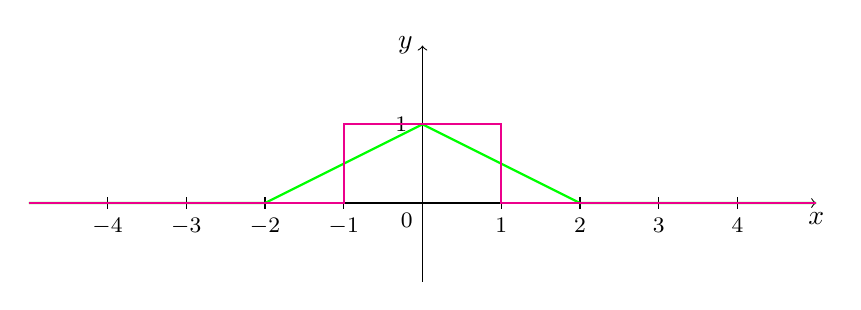
\begin{tikzpicture}
\draw[->] (-5,0) -- (5,0) node[below] {$x$};
\foreach \x in {-4,...,-1,1,2,...,4}
\draw[shift={(\x,0)}] (0pt,2pt) -- (0pt,-2pt) node[below] {\footnotesize $\x$};

\draw[->] (0,-1) -- (0,2) node[left] {$y$};
\foreach \y in {1}
\draw[shift={(0,\y)}] (2pt,0pt) -- (-2pt,0pt) node[left] {\footnotesize $\y$};
\node[below left] at (0,0) {\footnotesize $0$};

\draw[green,thick] (-5,0) -- (-2,0) -- (0,1) -- (2,0) -- (5,0);
\draw[magenta,thick] (-5,0) -- (-1,0) -- (-1,1) -- (1,1) -- (1,0) -- (5,0);
\end{tikzpicture}
\caption{Box filter and tent filter.}%
\label{fig:filters}
\end{figure}

Both filters discussed above can be interpreted as to particular members of a
larger family of (non-interpolating) B-splines. Note that $\Pi^n$ is only
interpolating for $n \le 2$; thus B-splines of higher order are smoothing
filters but not interpolating filters. One way to look at these filters is as
follows. We begin by expressing the interpolated continuous signal by a finite
number of continuous filters multiplied with a discrete coefficient, \ie a
scalar
\begin{equation*}
  g^c(l) = \sum_i c_i b(l)\,.
\end{equation*}
As mentioned above, if $b(l)$ is a B-spline of higher order, it is not
interpolating and thus, we need to account for this by choosing the coefficients
$c_i$ accordingly. If we want the signal to interpolate, the left and right hand
sides of the equation above must be equal at the interpolation points. If we
again write the filter as a Toeplitz matrix, this means that $g = Bc$ has to
hold (here we collected the $c_i$ into a vector). Solving for $c$ yields
\begin{equation*}
  c = B^{-1}g\,.
\end{equation*}
Of course, in general the matrix inversion is very expensive. Using the fact
that $B$ (and also its inverse) is Toeplitz, the inversion can be implemented in
terms of an infinite impulse response filter (IIR). This gives rise to so called
cardinal B-splines. Another approach which tries to approximate $\sinc$
resampling is the Lanczos filter. The methods discussed above can also be
regarded as computationally efficient approximations to Lanczos resampling.

Note that the ``subjectively'' best filter in general depends on the content of
the image. While in some cases the $\sinc$ might be the best choice, sometimes
the bilinear filter might produce better results. Thus, we would ideally like a
filter that adapts to the image content, \eg a neural network.

%%% Local Variables:
%%% mode: latex
%%% TeX-master: "../main"
%%% End:
